\documentclass[10pt, letterpaper]{article}
\usepackage[english]{babel}
\usepackage[utf8]{inputenc}

% Adding images
\usepackage{graphicx}
\usepackage{subcaption}

\title{Homework Heuristic Search}
\author{Calogero Carlino, 302154}
\date{\today}

\begin{document}
\maketitle

\section{Introduction}
The code developed for this assignment includes an \texttt{Agent} python 
class in which the functions for the 
\texttt{best\_first}, \texttt{a\_star}, \texttt{dfs} and 
\texttt{path\_follower} algorithms are implemented.

The heuristic definitions that can be used for the 
\texttt{best\_first} and the \texttt{a\_star} algorithm are the 
\texttt{manhattan\_distance\_euristic} and the 
\texttt{euclidean\_distance\_euristic}.

The maze on which these algorithms are applied can be generated with
a \texttt{backtracking} algorithm or a \texttt{randomized} one. In the 
randomized version, a path from goal to exit is always guaranteed
to exist even though obstacles are randomly generated.

Lastly, there are several \texttt{game} modules that can be executed, one
for every combination of algorithm and maze generation. Every game module
creates a new window in which the agent is animated while it moves toward
the goal.

\section{Comparative statistics}
Each algorithm was tested 80 times in a 10x10 room, one for every 
newly added obstacle in the maze, starting with a maze with no obstacles 
and ending with one made by 80 obstacles.

The graphs shown in \emph{Picture \ref{fig:maze_runner_algorithms_80_test_runs}} were produced out of the test data.

\begin{figure}[h]
    \centering
    \begin{subfigure}[b]{0.475\textwidth}
      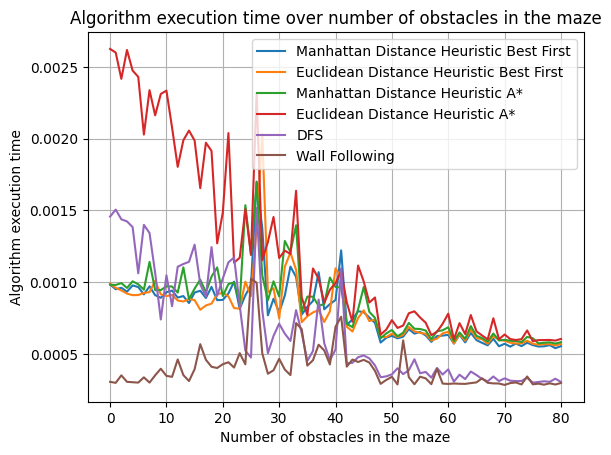
\includegraphics[width=\textwidth]{images/execution_time_test_graph.png}
      \caption{Execution time of each algorithm over the increasing number of obstacles in the maze}
      \label{execution_time_test_graph}
    \end{subfigure}
    \hfill
    \begin{subfigure}[b]{0.475\textwidth}
      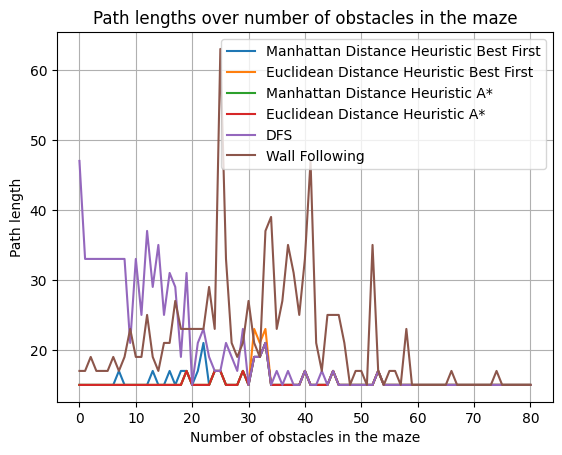
\includegraphics[width=\textwidth]{images/path_length_test_graph.png}
      \caption{Path length per algorithm over the increasing number of obstacles in the maze}
      \label{path_length_test_graph}
    \end{subfigure}
    
    \medskip % create some *vertical* separation between the graphs
    
    \begin{subfigure}[b]{0.475\textwidth}
      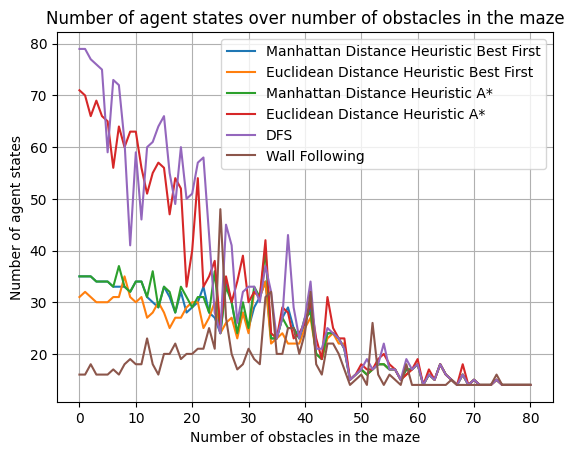
\includegraphics[width=\textwidth]{images/number_of_agent_states_test_graph.png}
      \caption{Number of agent states per algorithm over the increasing number of obstacles in the maze}
      \label{number_of_agent_states_test_graph}
    \end{subfigure}
    \hfill
    \begin{subfigure}[b]{0.475\textwidth}
      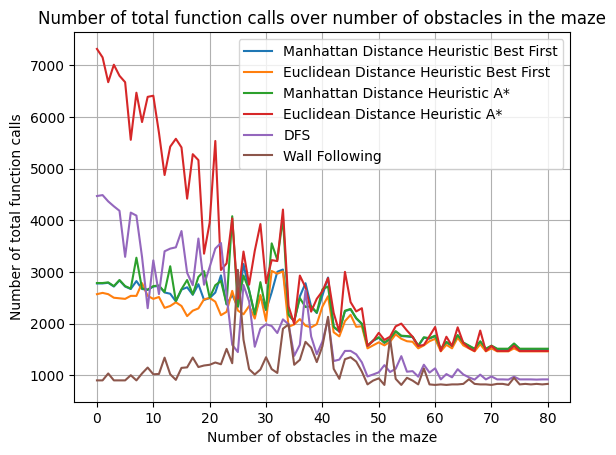
\includegraphics[width=\textwidth]{images/number_of_total_function_calls_test_graph.png}
      \caption{Number of total function calls per algorithm over the increasing number of obstacles in the maze}
      \label{number_of_total_function_calls_test_graph}
    \end{subfigure}
    
    \caption{Graphs derived by testing maze runner algorithms 80 times in a room with increasing obstacles}
    \label{fig:maze_runner_algorithms_80_test_runs}
\end{figure}

\section{Conclusions}
Having seen four different algorithms for solving the generated 
\texttt{10x10} maze (DFS, Wall Following, Best-First Search, and A*) we 
can conclude that DFS, Wall Following and Best-first Search are not guaranteed to 
find optimal solutions. While DFS can quickly find a solution, it is 
not necessarily the shortest one. The same can be said for the Wall 
Following algorithm, which is simple to implement; meanwhile the 
solution provided by the Best-first Search algorithm strongly depends 
on the quality of the heuristic function. Lastly, A* is optimal if the 
heurstic function is consistent (monotonically increasing).

Regarding time complexity, DFS has \texttt{O(|V| + |E|)} in the worst case, 
where \texttt{|V|} is the number of vertices and \texttt{|E|} is the number of edges. 
Wall Following has a worst-case time complexity of \texttt{O($n^{2}$)}, as it may 
explore every cell in an \texttt{n x n} maze. Best-first Search varies based on 
the heuristic and the problem and A* is exponential in the worst case 
but often performs much better inm pratice with a good heuristic.

Space complexity is also a factor to consider when comparing algorithms. 
Wall Following has \texttt{O(1)} space complexity because it only needs to store 
information about the current position and the direction of the wall 
it's following. DFS has a space complexity of \texttt{O(|V|)} in the worst case, 
while Best-first Search can vary widely, depending on the implementation 
and the heuristic function and A* is exponential in the worst case.

To summarize:
\begin{itemize}
    \item the DFS algorithm is good for finding a solution quickly, 
    but may not be optimal, so it can be used when the search space 
    is finite and the depth of the solution is known to be relatively 
    small;
    \item Wall Following is a simple strategy that can be applyed in 
    specific scenarios;
    \item Best-first can be faster than DFS, but less reliable, 
    meaning that it could be used when a good heuristic function 
    is available;
    \item A* is often the best choice for finding optimal solutions
    efficiently, so it can be used when a good heuristic function is 
    available and the search space is large.
\end{itemize}

\end{document}